\chapter{Partcle-grid-particle}
\section{Overview}
    Deep learning methods have been widely applied in computer vision, like segmentation, objects recognition. And training data is always crutial to the whole learning process. Normally, researchers prefer using the original image as the input images for training. However, it is still not clear that what kind of data can be used for predictiting the motion of onjects. Researchers in DeepMind\footnote{\url{https://deepmind.com/}} found that when deep neural networks are applied in physics motion prediction, the most difficult thing is to recognize different objects and get time-state data, like $m$, $\pmb{v}$, $\pmb{q}$, etc. In their new paper, they provide different colors to different moving bodies and use a sequence of frames as training data to make deep neural networks get state information($\pmb{v}, m, \pmb{q}$) \cite{DBLP:journals/corr/WattersTWPBZ17}.  Although visual interact networks work well to predict physics motion, it would be confused when it is facing many bodies dynamic system. In our view, we do not need deep learning model(e.g. convolutional neural networks) to replace the contact solver completely. We only hope deep neural network can accelerate the simulation. The learning model can give reasonable values which are close to the final solutions. Afterward, the iterative contact solver will use the values as starting, and ideally coverage rapidly. \\

    After discussion, we decided to transform each time-state to a grid map by Smoothed Particle Hydrodynamics. Then we will use the grid maps as the training data for deep learning model. Overall, the advantages of using the grid-based method are,
    \begin{enumerate}
        \item Grid map can describe the mass distribution so that neural networks can understand the distribution of objects. In other words, it is possible for deep neural networks to recognize the objects in the simulation.
        \item Grid map image can restore assessable data(mass, linear velocity, angular velocity) for deep learning neural networks, while the visualization image of simulation can only describe the position of rigid. This is helpful deep neural networks to find the relationship between state and contact forces.
    \end{enumerate}

    The basic method for generating training data which is more accessible to learning is that we will map a discrete element method(DEM) into a continuum setting use techniques from smooth particle hydrodynamics. Given a set of bodies $\mathcal{B}$ and a set of contacts between these bodies $\mathcal{C}$. The work process is like,
    \begin{enumerate}
        \item Based on Smoothed Particle Hydrodynamics(SPH), map current state($m, v_x, v_y, \omega, n_x$) to a image(the number of channel is 5.), which is called \textit{feature image}
        \item The \textit{feature image} will be used as input to a model(created by a convolutional neural network and introduced in Chapter \ref{cp:dp}), then one image(the number of channels is 2) will be got, which can be called \textit{label image}.
        \item For all contacts positions, interpolated values will be generated based on \textit{label image}. Then, the values will be used as starting iterate values for contact force solver. In our hypothesis, the given starting values will speed up the solver to reach convergence.
    \end{enumerate}

    \begin{figure}
        \centering
        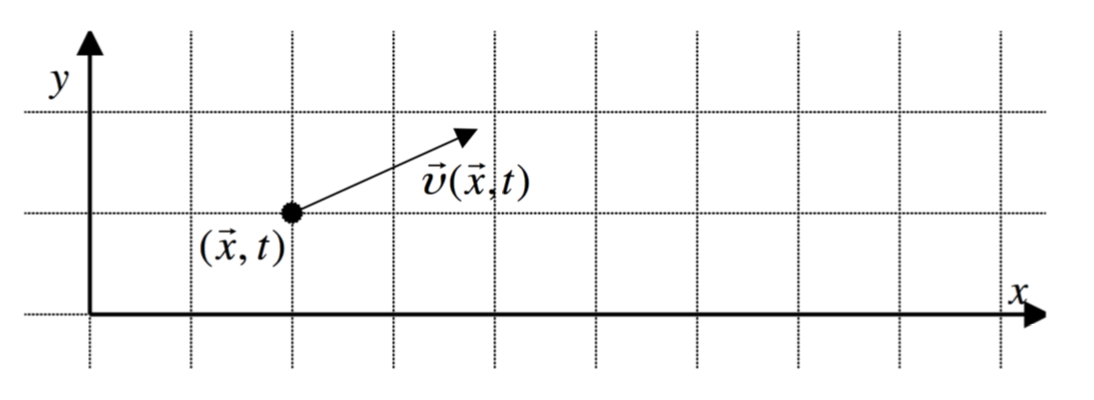
\includegraphics[scale = 0.4]{Figures/grid_method.png}
        \caption{Grid description, \textit{retrieved from MIT}(2011)}
    \end{figure}

\section{Smoothed Particle Hydrodynamics}
    Smoothed particle hydrodynamics (SPH) was invented to simulate nonaxisymmetric phenomena in astrophysics initially \cite{DBLP:journals/corr/GuWKMSSLWW15}. The principal idea of SPH is to treat hydrodynamics in a completely mesh-free fashion, in terms of a set of sampling particles. It turns out that the particle presentation of SPH has excellent conservation properties, energy, linear momentum, angular momentum, mass, and velocity.

    \subsection{Fundamentals}

    The heart of SPH is a kernel interpolation method which allows any function to be expressed in terms of its values at a set of disordered points - the particles\cite{monaghan1992smoothed}. For ant field $A(\textbf{r})$, a smoothed interpolated version $A_{I}(\textbf{r})$ can be defined by a kernel $W(\textbf{r}, h)$,
    \begin{equation}
        A_{I}(\textbf{r}) = \int A({\textbf{r}}^{\prime})W(\|\textbf{r} - \textbf{r}^{\prime}\|, h)\dif\textbf{r}^{\prime}
    \end{equation}
    \begin{figure}[!ht]
        \centering
        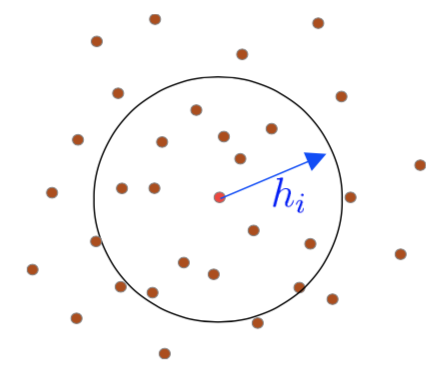
\includegraphics[scale = 0.6]{Figures/sph}
        \caption{Visilaztion of SPH}
    \end{figure}

    where the integration is over the entire space, and $W$ is an interpolating kernel with 
    \begin{equation}
        \int W(\|\textbf{r} - \textbf{r}^{\prime}\|, h)\dif \textbf{r}^{\prime} = 1
    \end{equation}
    and
    \begin{equation}
        \lim_{h\to 0} W(\|\textbf{r} - \textbf{r}^{\prime}\|, h)\dif\textbf{r}^{\prime} = \delta(\|\textbf{r} - \textbf{r}^{\prime}\|) 
    \end{equation}

    Normally, we want the kernel to be non-negative and rotational invariant, which can be written mathematically
    \begin{subequations}
        \begin{align}
            & W(\|\textbf{x}_{i} - \text{x}_{j}\|, h) = W(\|\text{x}_{j} - \text{x}_{i}\|, h) \\
            & W(\|\textbf{r} - \textbf{r}^{\prime}\|, h) \ge 0
        \end{align}
    \end{subequations}

    For numerical work, we can use the midpoint rule,
    \begin{equation}
        A_{I}(\textbf{x}) \approx A_{S}(\textbf{x}) = \sum_{i} A(\textbf{x}_{i})W(\|\textbf{x}_{i}-\textbf{x}\|, h)\Delta V_{i}
    \end{equation}
    Since $V_{i} = m_{i}/\rho _{i}$
    \begin{equation}
        A_{S}(\textbf{x}) = \sum_{i} \frac{m_{i}}{\rho_{i}} A(\textbf{x}_{i})W(\|\textbf{x}_{i}-\textbf{x}\|, h)
    \end{equation}

    The default, gradient and Laplacian of $A$ are:
    \begin{subequations}
        \begin{align}
            \nabla A_{S}(\textbf{x}) &= \sum_{i} \frac{m_{i}}{\rho_{i}} A(\textbf{x}_{i})\nabla W(\|\textbf{x}_{i}-\textbf{x}\|, h) \\
            \nabla^{2} A_{S}(\textbf{x}) &= \sum_{i} \frac{m_{i}}{\rho_{i}} A(\textbf{x}_{i})\nabla^{2} W(\|\textbf{x}_{i}-\textbf{x}\|, h)
        \end{align}
        \label{eq:1}
    \end{subequations}

    \subsection{Smoothing Kernels}
    \label{sec:kernels}
    Smoothing kernels function $W$ is one of the most important points in SPH. Stability, , and speed of the whole method depend on these functions. For different purposes, researchers will normally determine different kernels. One possibility for $W$ is a Gaussian. However, most current SPH implementations are based on kernels with finite support. So, I mainly introduce \textbf{poly6} and \textbf{spiky} kernels here. In the chapter \ref{details}, I will compare the different kernels and analyze which one is better.

    \subsubsection{Poly6}
    \label{poly6}
    The kernel is also known as the 6th degree polynomial kernel.
    \begin{equation}
        W_{poly 6}(\textbf{r}, h) = \frac{315}{64\pi h^{9}}
            \begin{cases}
                (h^2 - \|\textbf{r}\|^2)^3 & 0 \le \|\textbf{r}\| \le h \\
                0 & \textrm{Otherwise}
            \end{cases}
    \end{equation}

    Then, the gradient of this kernel function can be
    \begin{equation}
        \nabla W_{poly 6}(\textbf{r}, h) = - \frac{945}{32\pi h^9}
            \begin{cases}
                \textbf{r}(h^2 - \|\textbf{r}\|^2)^2 & 0\le\|\textbf{r}\|\le h \\
                0 & \textrm{Otherwise}\\
            \end{cases}
    \end{equation}

    The Laplacian of this kernel can be expressed by, 
    \begin{equation}
        \nabla^2 W_{poly6}(\textbf{r}, h) = - \frac{945}{16\pi h^9}
            \begin{cases}
                (h^2 - \|\textbf{r}\|^2)(3h^2-7\|\textbf{r}\|^2) & 0\le\|\textbf{r}\|\le h \\
                0 & \textrm{Otherwise}\\
            \end{cases}
    \end{equation}

    SPH is normally used in the liquid simulation. M\"uller suggested in \cite{muller2003particle}, this kernel can be used for the computation of pressure forces. Particles tend to build cluster under high pressure because `as particles get very close to each other, the repulsive force vanishes because the gradient of the kernel approaches zero to the center.'. We can see that in Figure \ref{fg:gradient}. Another similar kernel, spiky kernel, is proposed by Desbrum and Gascuel\cite{desbrun1996smoothed} to solve this problem.

    \subsubsection{Spiky}

    The kernel proposed by Desbrum and Gascuel\cite{desbrun1996smoothed}
    \begin{equation}
        W_{spiky}(\textbf{r}, h) = \frac{15}{\pi h^6}
            \begin{cases}
                (h - \|\textbf{r}\|)^3 & 0\le\|\textbf{r}\|\le h \\
                0 & \textrm{Otherwise}\\
            \end{cases}
    \end{equation}

    Then, the gradient of the spiky kernel can be described by,
    \begin{equation}
        \nabla W_{spiky}(\textbf{r}, h) = -\frac{45 \textbf{r}}{\pi h^6 \|\textbf{r}\|}
            \begin{cases}
                (h - \|\textbf{r}\|)^2 & 0\le\|\textbf{r}\|\le h \\
                0 & \textrm{Otherwise}\\
            \end{cases}
    \end{equation}
     The laplacian of spiky can be expressed by,
     \begin{equation}
        \nabla^2 W_{spiky}(\textbf{r}, h) = \frac{90}{\pi h^6}
            \begin{cases}
                h - \| \textbf{r} \| & 0 \le \| \textbf{r} \| \le h \\
                0 & \textrm{Otherwise}\\
            \end{cases}
    \end{equation}

    \begin{figure}[!ht]
        \centering
        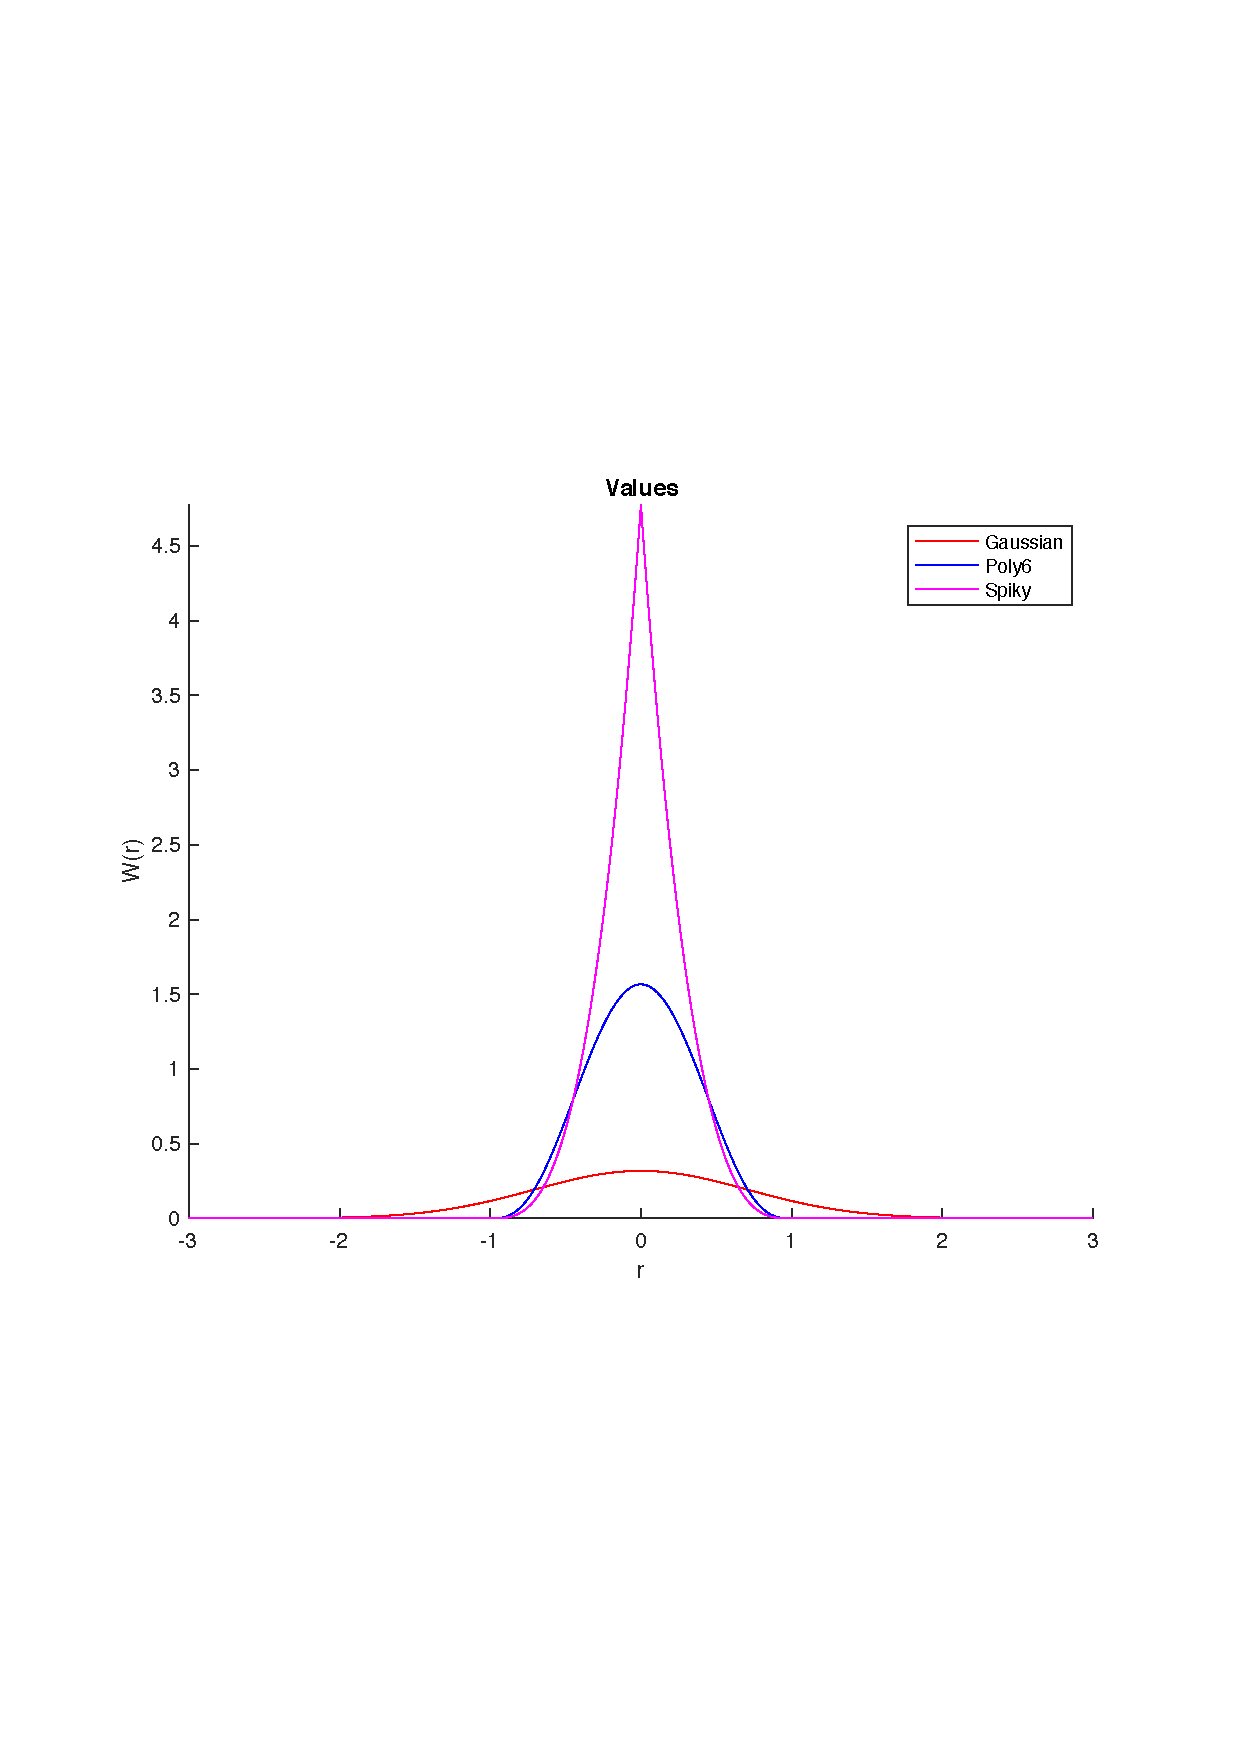
\includegraphics[scale = 0.5]{Figures/kernels}
        \caption{Comparation of different kernels, we set smoothing length $h = 1$ here.}
    \end{figure}

    \begin{figure}[!ht]
        \centering
        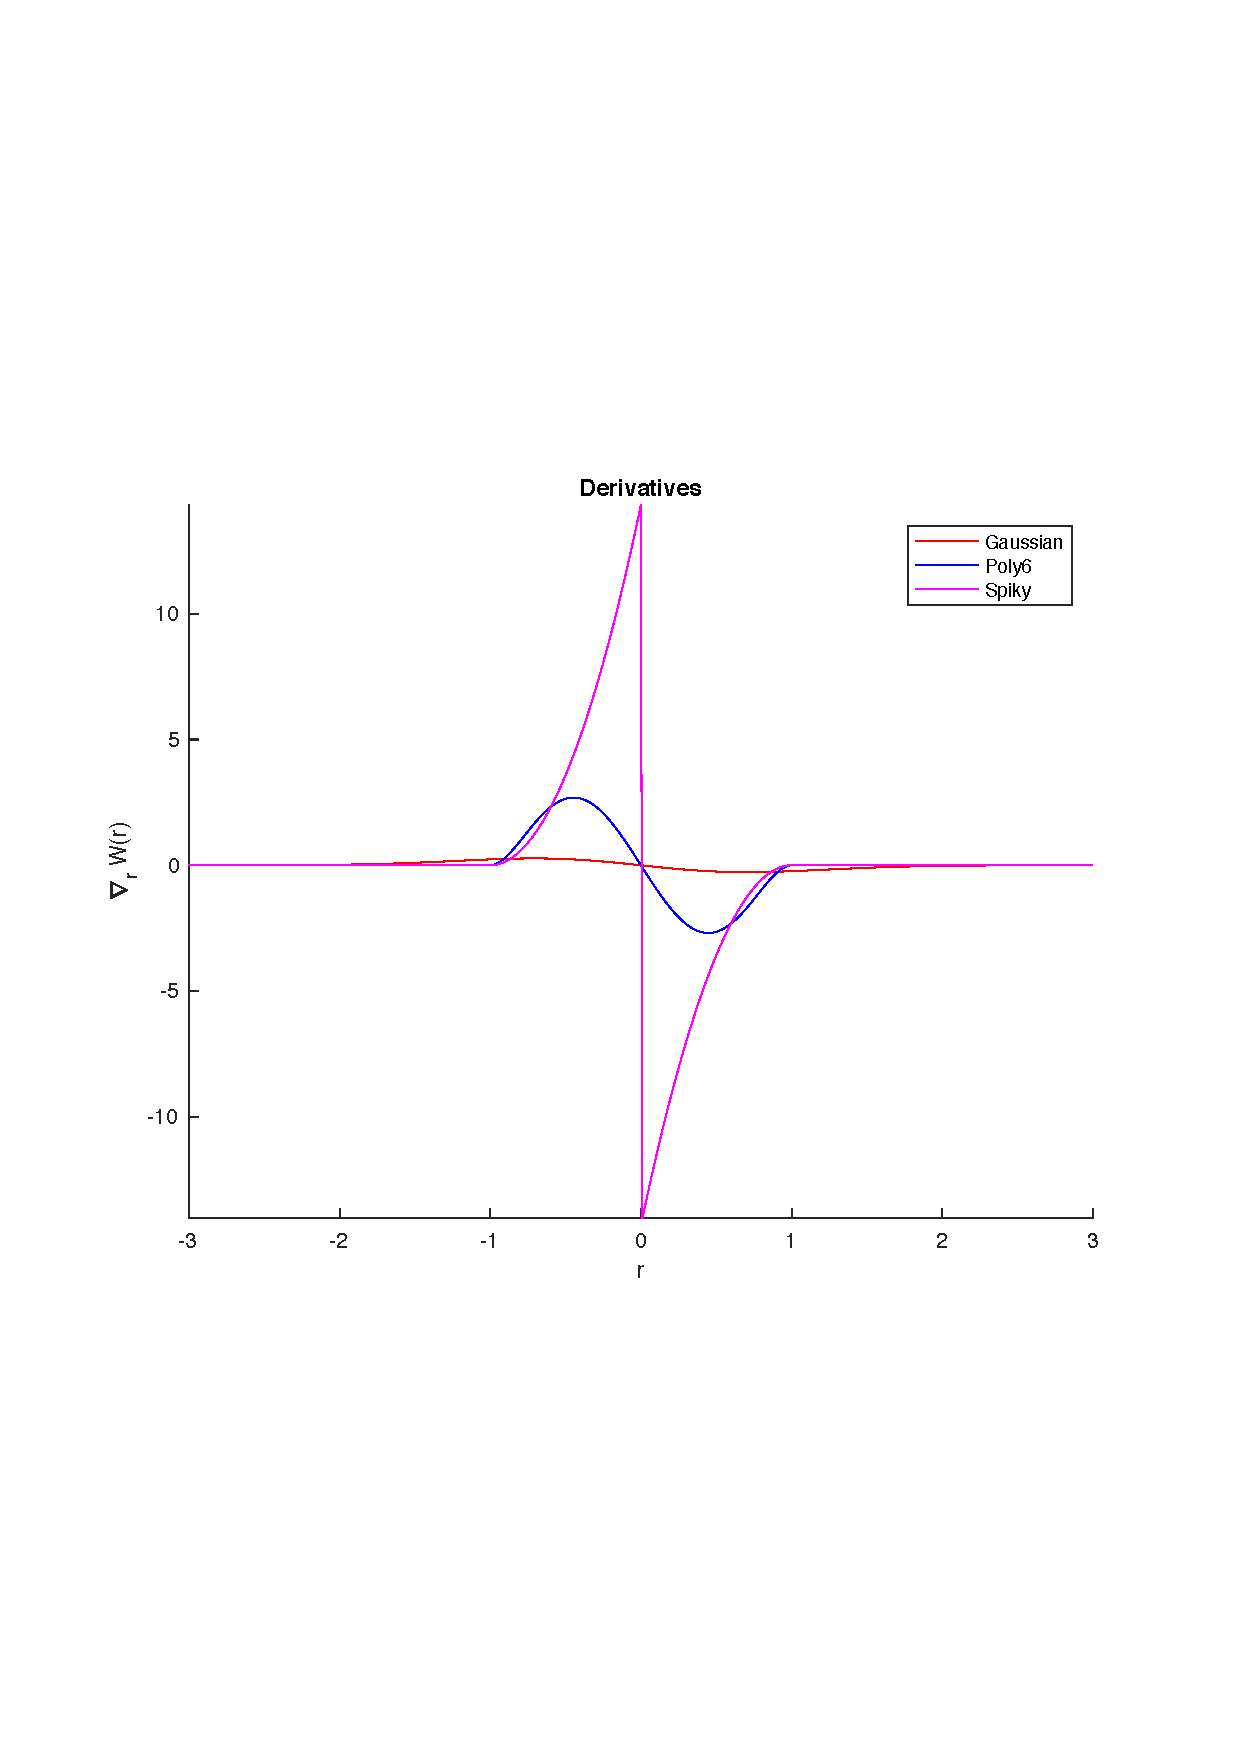
\includegraphics[scale = 0.5]{Figures/kenels_de}
        \caption{Comparation of gradient of different kernels, we set $h = 1$ here. }
        \label{fg:gradient}
    \end{figure}

    \subsection{Grid size and smoothing length}
    \label{gs}
    The grid should be also fine enough to capture the variation in our simulation. In this case, it is reasonable to have a grid fine enough such that no two contact points are mapped into the same cell. \\

    Smoothing length, $h$, is another one of the most important parameters, which affects the whole SPH method by changing the kernel value results and neighbor searching results. Too small or too big values might cause lose essential information in the simulation.

    \subsection{Neighbor Search}
    Neighbor search is one of the most crucial procedures in SPH method considering all interpolation equations, $A(\textbf{r})$, needs the neighbor list for every particle (refer to equation \ref{eq:1}). A naive neighbor searching approach would end up with a complexity of $O(n^2)$. The complexity is not good enough since it is impossible to reach any interactive speed when the particle count increases. It is possible to have a significant performance increase with using an efficient nearest neighbor searching(NNS), since NNS is the most time-consuming process in SPH computation. In order to decrease the complexity, we choose to use $k-d$ tree data structure to store the particle spatial information and then do the nearest neighbor searching. $k-d$ tree is a data structure proposed by Bentley and Jon \cite{bentley1975multidimensional}, and we will use the $k-d$ algorithm built in \textit{Scipy}\footnote{\url{https://docs.scipy.org/doc/scipy-0.14.0/reference/generated/scipy.spatial.KDTree.html}}

    \subsection{Summary}
    Then, I can conclude the whole process for map current simulation state to grid images,
    \begin{algorithm}[!h]
        \KwData{
            Given a set of bodies $\mathcal{B}$ and the state in time $t$, as well as all grid nodes $\mathbf{x}$
        }
        \KwResult{the body grid image $\pmb{G}_{\mathcal{B}}(\mathbf{x})$}
        \For{all $i$ and $j$}{
            1. Find the nearest neihbors $\mathcal{B}_{near} \subseteq \mathcal{B}$ around $\mathbf{x}_{ij}$ \;
            2. read the current state,
                $$m_k, \pmb{v}_k, \pmb{q}_k, \omega_{k}~~k\in\mathcal{B}_{near}$$
            3. Define state vector 
                $$\pmb{S}_{k} = [m_k, {v_k}_{x}, {v_k}_{y}, \omega_{k}]$$
            4. Compute grid values
                $$\pmb{G}_{\mathcal{B}}(\mathbf{x}_{ij}) = \sum_{k\in \mathcal{B}_{near}}W(\mathbf{x}_{ij}, \pmb{q}_{k})\pmb{S}_k$$
        }
        \caption{Mapping bodies into a grid image. $\pmb{G}_{\mathcal{B}}=Bodies2grid(\mathbf{x}, \mathcal{B})$}
        \label{bodygrid}
    \end{algorithm}

    \begin{algorithm}[!h]
        \KwData{Given a set of contacts $\mathcal{C}$ between a set of bodies $\mathcal{B}$ and the state in time $t$, as well as all grid nodes $\mathbf{x}$}
        \KwResult{the contact grid image $\pmb{G}_{\lambda}(\mathbf{x})$}
        \For{all $i$ and $j$}{
            1. Find the nearest neihbors $\mathcal{C}_{near} \subseteq \mathcal{C}$ around $\mathbf{x}_{ij}$ \;
            2. read the current contact forces values and its position.
                $$\pmb{q}_k, \pmb{\lambda}_{k}~~k\in\mathcal{C}_{near}~~\pmb{\lambda} = [\lambda_n, \lambda_t]$$
            3. Compute grid values
                $$\pmb{G}_{\lambda}(\mathbf{x}_{ij}) = \sum_{k\in \mathcal{C}_{near}}W(\mathbf{x}_{ij}, \pmb{q}_{k})\pmb{\lambda}_k$$
        }
        \caption{Mapping contacts into a grid image. $\pmb{G}_{\lambda}=Contacts2grid(\mathbf{x}, \mathcal{C})$}
        \label{contactgrid}
    \end{algorithm}


\section{Grid to particle}
    SPH will be used for us to transform current state of dynamic system to grid images. After obtaining the grid image for simulation state in time $t$, we will use the grid cells as input and renew the contact grid image based on trained model. After getting the contact force grid image, the next step is to use contact position to interpolate image values. The interpolated values will be stored in the contact points and used as starting iterates for contact force solver. Then we can update states of all rigid bodies in time $t+\Delta{t}$.

    \subsection{Bilinear interpolation}
    We applied bilinear interpolation in our case, since we did mainly research on a rectilinear $2-D$ grid.
    \begin{figure}
        \centering
        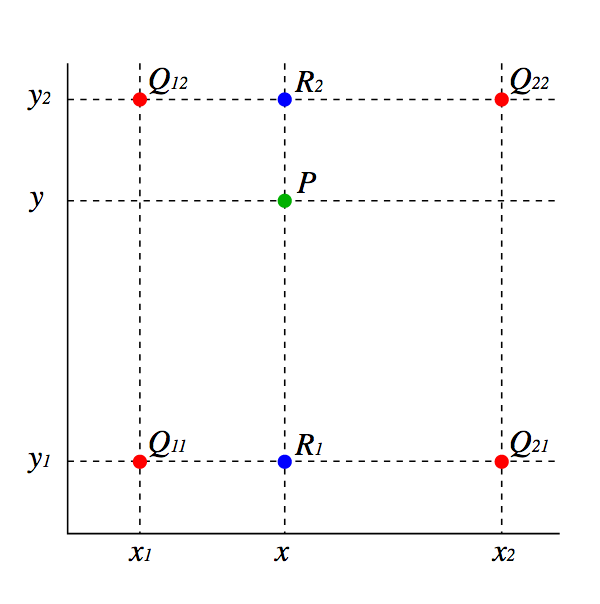
\includegraphics[scale = 0.8]{Figures/inp}
        \caption{The figure shows the visualization of bilinear interpolation. The four red dots show the data points and the green dot is the point at which we want to interpolate.}
        \label{fig:1}
    \end{figure}
    The key idea is to perform linear interpolation first in one direction, and then again in the other direction. Although each step is linear in the sampled values and in the position, the interpolation as a whole is not linear but rather quadratic in the sample location. \\

    As shown in Figure \ref{fig:1}, We have known $Q_{a, b} = (x_a, y_ b)$ and $a\in\{1, 2\}\quad b\in\{1,2\}$. Then, we can firstly do linear interpolation in the $x$-direction. This yields

    \begin{subequations}
        \begin{align}
            f(x,y_{1})&\approx {\frac {x_{2}-x}{x_{2}-x_{1}}}f(Q_{11})+{\frac {x-x_{1}}{x_{2}-x_{1}}}f(Q_{21}),\\
            f(x,y_{2})&\approx {\frac {x_{2}-x}{x_{2}-x_{1}}}f(Q_{12})+{\frac {x-x_{1}}{x_{2}-x_{1}}}f(Q_{22}).
        \end{align}
        \label{eq:2}
    \end{subequations}

    After getting the two values in $x-$direction $f(x, y_1)$ and $f(x, y_2)$, we can combine these values to do interpolation in $y-$ direction.
    \begin{equation}
        f(x,y) \approx {\frac {y_{2}-y}{y_{2}-y_{1}}}f(x,y_{1})+{\frac {y-y_{1}}{y_{2}-y_{1}}}f(x,y_{2})
    \end{equation}

    Combine $f(x, y_1)$ and $f(x, y_2)$ defined in equation \ref{eq:2}, we can get,

    \begin{equation}
        \begin{aligned}
        f(x,y)&\approx{\frac {y_{2}-y}{y_{2}-y_{1}}}\left({\frac {x_{2}-x}{x_{2}-x_{1}}}f(Q_{11})+{\frac {x-x_{1}}{x_{2}-x_{1}}}f(Q_{21})\right)\\&\qquad+{\frac {y-y_{1}}{y_{2}-y_{1}}}\left({\frac {x_{2}-x}{x_{2}-x_{1}}}f(Q_{12})+{\frac {x-x_{1}}{x_{2}-x_{1}}}f(Q_{22})\right)\\&={\frac {1}{(x_{2}-x_{1})(y_{2}-y_{1})}}{\big (}\\&\qquad f(Q_{11})(x_{2}-x)(y_{2}-y)+f(Q_{21})(x-x_{1})(y_{2}-y)\\&\qquad+f(Q_{12})(x_{2}-x)(y-y_{1})+f(Q_{22})(x-x_{1})(y-y_{1}){\big )}\\&={\frac {1}{(x_{2}-x_{1})(y_{2}-y_{1})}}{\begin{bmatrix}x_{2}-x&x-x_{1}\end{bmatrix}}\\&\qquad \cdot {\begin{bmatrix}f(Q_{11})&f(Q_{12})\\f(Q_{21})&f(Q_{22})\end{bmatrix}}{\begin{bmatrix}y_{2}-y\\y-y_{1}\end{bmatrix}}
        \end{aligned}
        \label{interpolation}
    \end{equation}

    Then, the bilinear interpolation algorithm can be summarized,
    \begin{algorithm}[!h]
        \KwData{A grid image $\pmb{G}$, position $\pmb{q}$}
        \KwResult{the contact grid image $\pmb{G}_{\lambda}(\mathbf{x})$}
        \For{all $i$ and $j$}{
            1. Find the nearest neihbors $\mathcal{C}_{near} \subseteq \mathcal{C}$ around $\mathbf{x}_{ij}$ \;
            2. read the current contact forces values and its position.
                $$\pmb{q}_k, \pmb{\lambda}_{k}~~k\in\mathcal{C}_{near}~~\pmb{\lambda} = [\lambda_n, \lambda_t]$$
            3. Compute grid values
                $$\pmb{G}_{\lambda}(\mathbf{x}_{ij}) = \sum_{k\in \mathcal{C}_{near}}W(\mathbf{x}_{ij}, \pmb{q}_{k})\pmb{\lambda}_k$$
        }
        \caption{Mapping contacts into a grid image. $\pmb{G}_{\lambda}=Contacts2grid(\mathbf{x}, \mathcal{C})$}
        \label{contactgrid}
    \end{algorithm}


\section{Experiment and Conclution}
    \label{sec:sph-exp}
    Our hope is that starting iterates will be close to ``solution'' of the contact problem, which can indicate the contact force solvers will coverage very rapidly or maybe not even need to iterate. In order to test whether the SPH method can be applied in our case, the contact force solution is mapped to image and interpolated values are generated and used to restart the contact force solver. Our hypothesis is that the iterative solver quickly recovers an iteration close to the original solution before mapping to force grid image. I will just compare the performance of SPH-based method with other methods in this section. More details will be analyzed and described in Chapter \ref{details}.

\subsection{pybox2d simulation}
    \label{sph:exp}
    In order to test whether \textbf{SPH-based} method works for this case. All experiments will be done based on the basis physical engine, \textit{pybox2d}. Before testing the performance of \textbf{SPH-based} method, \textbf{Non-model}, \textbf{Builtin-model} and \textbf{Copy-model} are defined to see the influence of different initial values for iterative contact solver.
    \begin{itemize}
        \item \textbf{Non-Model} In each step of the simulation, before the contact solver starts iteration to make a resolution for current dynamic system equation, the initial $\lambda_{f}$ and $\lambda_{t}$ of every contact will be given value $0$.
        \item \textbf{Builtin-Model} In each step of the simulation, before the contact solver starts iterations to make a resolution for current dynamic state equation, the initial value of $\lambda_f$ and $\lambda_{t}$ will be determined by the built-in algorithm. In other words, this model is the default solution built in \textit{pybox2d}.
        \item \textbf{Copy-Model} In each step of the simulation before the contact solver starts iteration to make a resolution for current dynamic system equation, the initial value of $\lambda_f$ and $\lambda_t$ will be the actual solution after exact iterations solver.
    \end{itemize}
    After defining these models, each model will be applied in the same rigid dynamic simulation process. The setting is given below,
    \begin{itemize}
        \item \textbf{World Setting}, the world box size is $30\times30$,   and there are $100$ circle rigids($r=1$, all circle rigid bodies in the same size.) inside the box. Initially, the rigid circles will be located following gaussian distribution\footnote{\url{https://en.wikipedia.org/wiki/Normal_distribution}}. Then, all rigid circles will fall down by gravity. The visualization of simulation is shown in Figure \ref{fig:simvi}.
        \item \textbf{Simulation Setting}, there will be totally $600$-steps simulation. For each step, $\Delta t = 0.01s$, and the number of iteration in each step will be set as fixed, $3000$. Then I will use the average convergence rate to show how fast the model coverages.
    \end{itemize}
    \begin{figure}[!h]
        \centering
        \begin{subfigure}[b]{0.3\textwidth}
            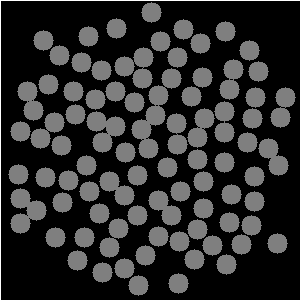
\includegraphics[width=\textwidth]{Figures/sim0.png}
            \caption{Time Step=$0$}
        \end{subfigure}
        \begin{subfigure}[b]{0.3\textwidth}
            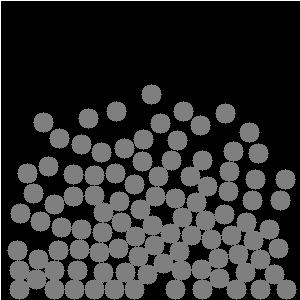
\includegraphics[width=\textwidth]{Figures/sim2.png}
            \caption{Time Step=$200$}
        \end{subfigure}
        \begin{subfigure}[b]{0.3\textwidth}
            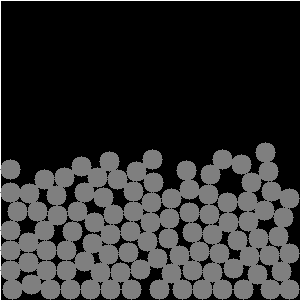
\includegraphics[width=\textwidth]{Figures/sim3.png}
            \caption{Time Step=$400$}
        \end{subfigure}
        \caption{Visualization for experiment simulation}
        \label{fig:simvi}
    \end{figure}
    \begin{figure}[!h]
        \centering
        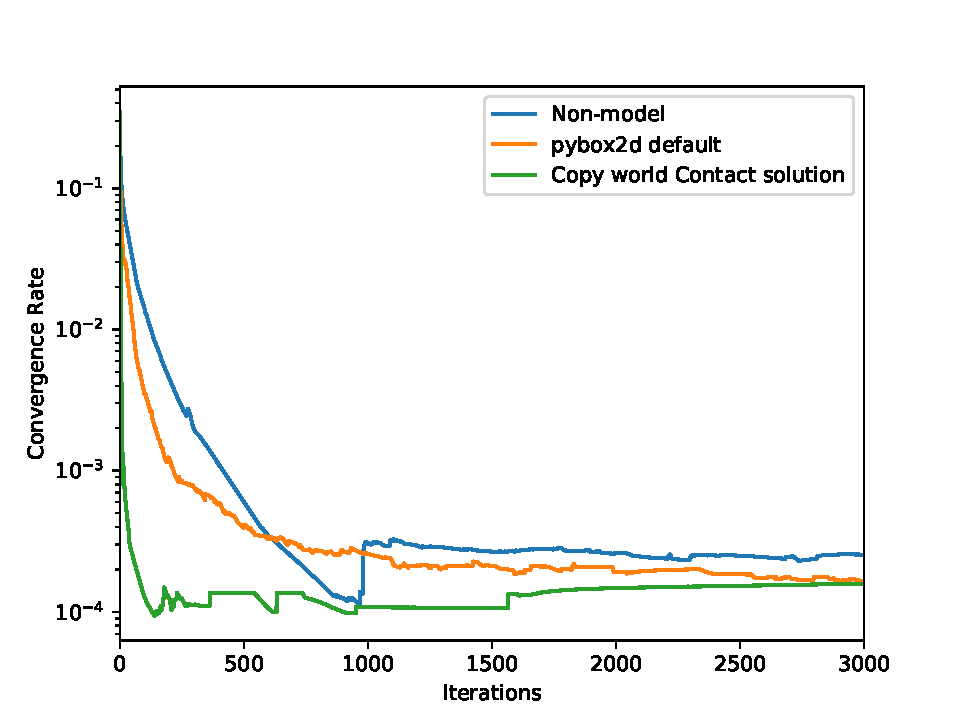
\includegraphics[width=\textwidth]{Figures/nosph}
        \caption{Average convergence rate for different models(not including \textbf{SPH-based model}).}
        \label{fg:nosph}
    \end{figure}
    The results are described in Figure \ref{fg:nosph}. Then, we can get some basic conclusions,
    \begin{itemize}
        \item \textbf{Copy-Model} performs the best, nearly no iteration to get convergence, since the correct solution would be given to the solver for start iterating.
        \item If all the starting values for iterative solver are zeros, it has to take a long time to reach convergence, which is indicated by \textbf{Non-Model}.
        \item The \textbf{Builtin-Model} performs similarly with \textbf{Non-Model}, far slower than \textbf{Copy-Model}.
    \end{itemize}
    Then, we can make a hypothesis,
    \begin{itemize}
        \item \textbf{Hypothesis} Ideally, if SPH-based method can work well for this project, the contact solver would coverage faster than \textbf{Builtin-Model} and \textbf{None-Model}, but still slower than \textbf{Copy-Model}, which give the correct solution to solver directly.
    \end{itemize}

\subsection{SPH-based method test}
    \label{sphtest}
    The \textbf{SPH-Model} is defined as follow, as well as the experiment algorithm in Algorithm \ref{testsph},
    \begin{itemize}
         \item \textbf{SPH-Model} In each step of simulation, one grid map $G(\mathbf{\pmb{\lambda}})~~\pmb{\lambda} = [\lambda_n, \lambda_t]$ will be created based on given rigid bodies $\mathcal{B}$ and contacts $\mathcal{C}$ between the bodies. Then, interpolated values would be generated by given contact point position $(x_j, y_j)~~j \in \mathcal{C}$ and would be used as initial values for iterative contact solver in \textit{pybox2D}. 
    \end{itemize}
    \begin{algorithm}[!h]
        \KwData{
            Given a set of bodies $\mathcal{B}$ and the state in time $t$, as well as some information of contacts between these bodies $\mathcal{C}$.
        }
        \KwResult{Get the contact forces $\pmb{\lambda}_{j}=[{\lambda_{n}}_{j}, {\lambda_{t}}_j]~~j\in\mathcal{C}$ at time $t$.}
        \While{Simulation Runing}
        {   1. map the solved contact to a gird image, $\mathbf{x}=(x_i, y_i)$ is the spatial position of one node in in grid image.
                $$\pmb{G}_{\lambda}=Contacts2grid(\mathbf{x}, \mathcal{C})$$
            2. Once the contact force image $\pmb{G}_{\lambda}$ is obtained,  the conatct position $\pmb{q}_{j} = (x_{j}, y_{j})~~j\in\mathcal{C}$  will be used to interpolation image values based on Equation \ref{interpolation}.
                $$\pmb{\lambda}_j \approx G_{\pmb{\lambda}}(\pmb{q}_j)~~j\in\mathcal{C}$$ 
            The interpolated values $\pmb{\lambda}$ will be used as restarting iterated for \textit{pybox2d} conatc solver. \\
            3. Update $t$
                $$t = t + \Delta t$$ \\
        }
        \caption{Experiment algorithm for test \textbf{SPH-Model}}
        \label{testsph}
    \end{algorithm}
    Finally, the plot about the 
    \begin{figure}[!h]
        \centering
        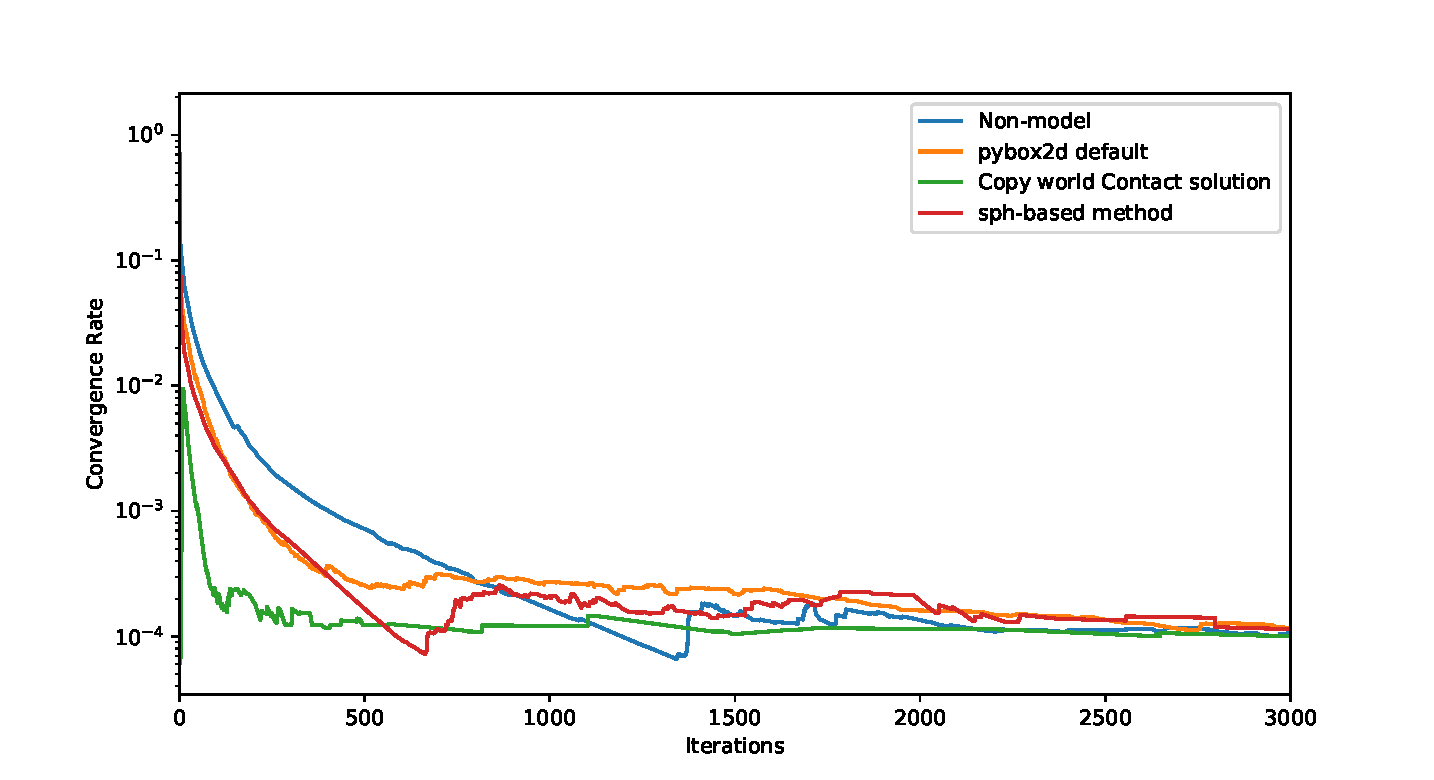
\includegraphics[width=\textwidth]{Figures/addsph}
        \caption{Convergence rate for different models(including \textbf{SPH-based model}).}
        \label{fg:addsph}
    \end{figure}
    As the hypothesis I supposed, \textbf{SPH-Model} converges faster than \textbf{Non-Model}. This can demonstrate the \textbf{SPH-based} method is a good strategy, which can make iterative contact solver converge quickly.

\subsection{Conclusion}
    Based the result in Figure \ref{fg:nosph} and \ref{fg:addsph}, it can be concluded that \textbf{SPH-based} strategy is available for the case in this thesis. Once the correct contact forces grid is achieved, the interpolated values will help the iterative solver to get convergence faster. So, the next step is to train an available model based on training data. The overall algorithm is concluded in Algorithm \ref{al:basic}.